\documentclass[12pt]{article}
%\usepackage{amsmath}
\usepackage{graphicx}
%\usepackage{enumerate}
\usepackage{natbib} %comment out if you do not have the package
\usepackage{url} % not crucial - just used below for the URL 
\usepackage{amsmath, amssymb}


%\pdfminorversion=4
% NOTE: To produce blinded version, replace "0" with "1" below.
\newcommand{\blind}{0}

% DON'T change margins - should be 1 inch all around.
\addtolength{\oddsidemargin}{-.5in}%
\addtolength{\evensidemargin}{-.5in}%
\addtolength{\textwidth}{1in}%
\addtolength{\textheight}{1.3in}%
\addtolength{\topmargin}{-.8in}%


\begin{document}

%\bibliographystyle{natbib}

\def\spacingset#1{\renewcommand{\baselinestretch}%
{#1}\small\normalsize} \spacingset{1}


%%%%%%%%%%%%%%%%%%%%%%%%%%%%%%%%%%%%%%%%%%%%%%%%%%%%%%%%%%%%%%%%%%%%%%%%%%%%%%

\if0\blind
{
  \title{\bf Computer model calibration as a method for design}
  \author{Carl Ehrett\thanks{
    The authors gratefully acknowledge \textit{please remember to list all relevant funding sources in the unblinded version}}\hspace{.2cm}\\
    School of Mathematical and Statistical Sciences, Clemson University,\\
    D. Andrew Brown \\
    School of Mathematical and Statistical Sciences, Clemson University,\\
    Evan Chodora \\
    Department of Mechanical Engineering, Clemson University,\\
    Mingzhe Jiang \\
    Department of Chemical and Biomolecular Engineering, Clemson University,\\
    Christopher Kitchens \\
    Department of Chemical and Biomolecular Engineering, Clemson University,\\
    and \\
    Sez Atamturktur \\
    Department of Architectural Engineering, Pennsylvania State University\\}
  \maketitle
} \fi

\if1\blind
{
  \bigskip
  \bigskip
  \bigskip
  \begin{center}
    {\LARGE\bf Title}
\end{center}
  \medskip
} \fi

\bigskip
\begin{abstract}
In traditional engineering design, material selection involves choosing a material with appropriate properties from a database of known materials, often as a matter of ad-hoc satisficing. 
Material design usually occurs separately, and without an eye to specific end-uses. We wed these design processes, selecting a material design by modeling its performance outcomes in a particular engineering application.
 We show that existing techniques for model calibration can be profitably reconceptualized as a method for optimization and applied to solve this material design problem. 
We demonstrate by calibrating material design parameters to desired performance targets for a wind turbine blade.
\end{abstract}

\noindent%
{\it Keywords:}  Uncertainty quantification, Gaussian processes, optimization, Pareto optimality, wind turbines, material design
\vfill

\newpage
\spacingset{2} % DON'T change the spacing!
\section{Introduction}
\label{introduction}

Broadly, in model calibration, one may consider a model to be of the form $\eta(\mathbf x,\boldsymbol \theta)$, where $(\mathbf x,\boldsymbol \theta)$ comprise all inputs to the model. 
%
Input vector $\mathbf x$ is the collection of inputs that are known and/or under the control of the researcher.
%
The vector of calibration inputs $\boldsymbol \theta$ is the collection of parameters the values of which are unknown. 
%
These must be estimated for successful simulation. 
%
Thus where $f$ describes the true system and $y$ an observation of that system, consider the model to be 
%
\begin{equation} \label{eq:model_gen}
y(\mathbf x)=f(\mathbf x)+\epsilon(\mathbf x)=\eta(\mathbf x,\boldsymbol \theta) + \delta(\mathbf x)+\epsilon(\mathbf x)
\end{equation} 
%
where $\delta(\cdot)$ describes the model discrepancy -- i.e., the bias of the model as an estimate of the real system -- and $\epsilon(\cdot)$ is a mean-zero observation error, often i.i.d.\ Gaussian. 
%

Much interest in the past two decades has centered on Bayesian methods for model calibration. 
%
The appeal of a Bayesian approach to model calibration is that the calibration parameters are a source of uncertainty for the model. 
%
This uncertainty should be quantified so that its effect on the model can be made explicit. 
%
One can use Bayesian methods to construct a posterior distribution of the calibration parameters which balances our prior knowledge about the calibration parameters with what can be learned from the available data, and which allows for accurate uncertainty quantification on the model outputs. 

In many cases of optimization, there are no unknown input parameters for the model. 
%
Instead, there are control inputs for which it is unknown which settings achieve optimality.
%
In the application studied here -- designing a composite material for a wind turbine blade -- the unknowns are the optimal ratio of the two ingredients of the composite and the optimal thickness of the material when used in a blade.
%
These unknown inputs can be treated as unknown parameters in a calibration problem.
%
Rather than calibrating a computer model's unknown parameters to observations from the real system, then, we calibrate the computer model's control input settings to performance targets.
%
The performance targets are treated as though they were observations of a real system, and the calibration minimizes the discrepancy between the computer model output and these ``desired observations.''
%
The proposed methodology provides not merely a point estimate of optimal settings, but a posterior distribution which includes uncertainty quantification.

The proposed methodology uses the Bayesian framework for computer model calibration provided by  \cite{Kennedy2001}.
% 
This area is furthered by \cite{Higdon2004}, who undertake model calibration with quantification of the related uncertainty. 
They explicitly incorporate uncertainty regarding the computer model output, the bias of the computer model, and uncertainty due to observation error (of field data). 
%
That approach is further refined and exemplified by \cite{Williams2006}.
%
\cite{Loeppky2006} offer an MLE-based alternative to the Bayesian approach promulgated by Kennedy and O'Hagan, intending thereby to improve the identifiability of the calibration parameters in the face of model discrepancy. 
%
\cite{Bayarri2007} extend the approach of Kennedy and O'Hagan, allowing for simultaneous validation and calibration of a computer model (using the same training data). 
%
\cite{Bayarri} apply this methodology to functional data using a hierarchical framework for the coefficients of a wavelet representation of the functional data. 
%
Similarly, \cite{Paulo2012} apply the lessons of \cite{Bayarri2007} to computer models with multivariate output.
%
\cite{Brynjarsdottir2014} demonstrate the importance of strong priors on the model discrepancy term when undertaking calibration.

Common to these approaches is the conception of calibration as a matter of aligning the computer model output to observations of the real system. 
%
In this paper, we calibrate a computer model to align with performance targets, in order to find system settings that optimize performance with respect to those targets.
%
In Section \ref{calib_for_design} we describe the calibration framework that we adapt as a method for optimization. 
%
In Sections \ref{example} and \ref{application} we apply the proposed methodology to an example involving simulated data and to an application in which the goal is to find material design settings to optimize the performance of a wind turbine blade.
%
In Section \ref{application} we also apply the methodology to produce an estimate of the entire Pareto front of the (trivariate) system (where the Pareto front is the set of inputs such that making any of the system outputs better off would require making one or more of the outputs worse off).
%
Section \ref{conclusion} concludes with discussion of the results.

\section{Calibration for design}\label{calib_for_design}
%\subsection{Calibration framework} \label{calib_framework}

In describing the calibration framework we use in this work, when an emulator is needed we assume the use of a Gaussian process (GP) emulator.
%
Just as a multivariate Gaussian random variable is characterized by its mean vector and covariance matrix, a Gaussian process is fully characterized by its mean function $\mu:D\to \mathbb R$ and covariance function $C:D\times D\to \mathbb R$, where $D$ is the domain of the process. 
%
Thus for any points $\mathbf x,\mathbf y$ in the domain of the Gaussian process, $\mu(\mathbf x)$ gives the mean of the Gaussian process at $\mathbf x$, and $C(\mathbf x, \mathbf y)$ gives the covariance between the values of the Gaussian process at points $\mathbf x$ and $\mathbf y$.
%
The distribution of the process at any finite number of points is multivariate Gaussian with mean vector and covariance matrix given by $\mu(\cdot)$ and $C(\cdot,\cdot)$.
%
In principle, model calibration need not rely on a GP emulator, or any other sort of emulator; one could (e.g.) complete a full Bayesian analysis via an MCMC chain that involves running the relevant computer model at each iteration of the chain. 
%
Indeed, in Section \ref{example} we perform calibration on our example simulated data without an emulator.
%
However, computer models are frequently too computationally expensive to allow for such profligacy.
%
Instead, a computationally tractable emulator can be constructed using a sample of observations from the computer model. 
%
GPs are popular prior distributions on computer model output for three reasons.
%
Firstly, because their use does not require detailed foreknowledge of the model function's parametric form. 
%
Secondly, GPs easily interpolate the computer model output, which is attractive when the computer model is deterministic. 
%
This is usually the case, although some attention in model calibration has focused specifically on stochastic computer models; see e.g.\ \cite{Pratola2018}. 
%
Thirdly, GPs facilitate uncertainty quantification through the variance of the posterior GP. 
%
This section provides brief background on Gaussian processes and their use in regression broadly and in computer model calibration specifically.
%

The use of GPs to produce a computationally efficient predictor $\hat \eta (\mathbf x)$ of expensive computer code $\eta(\mathbf x)$ given observations of code output at $\mathbf X=(\mathbf x_1,\ldots,\mathbf x_n)^T$ is promulgated by \cite{Sacks1989} and explored at length by \cite{Santner2003a}.
%
Since computer code is typically deterministic, these applications differ from the focus of \cite{OHagan1978} in that the updated GP is induced to interpolate the observations $\boldsymbol \eta = (\eta(\mathbf x_1),\cdots,\eta(\mathbf x_n))^T$. 
%
\cite{Kennedy2001} use GPs for computer model calibration. 
%
\cite{Kennedy2006} showcase this use of GP emulators for uncertainty and sensitivity analyses. 
%
\cite{Bastos2009} describe both numerical and graphical diagnostic techniques for assessing when a GP emulator of a computer model is successful, as well as discussion of likely causes of poor diagnostic results. 
%
While most work in the area of GP emulation uses stationary covariance functions (in which $\mu(\cdot)$ is constant and $C(\mathbf x,\mathbf x' )\equiv C(\mathbf x-\mathbf x' )$ depends only on the difference between $\mathbf x$ and $\mathbf x'$, rather than on their location in the input domain) and quantitative inputs, efforts have been made to branch away from these core uses. 
%
\cite{Gramacy2008} use treed partitioning to deal with a nonstationary computer model. 
%
\cite{Qian2008} explore methods for using GP emulators that include both quantitative and qualitative inputs.
%

Suppose that we have inputs $\{\mathbf x_i\}_{i=1}^n\subseteq \mathbb R^p$ scaled to the unit hypercube, and observations 
%
%\begin{equation}\label{eq:2}
$y(\mathbf x_i) = f(\mathbf x_i) + \epsilon(\mathbf x_i),$ for $i=1,\cdots,n,$
%\end{equation}
%
where $f(\cdot)$ is the true system and $\epsilon(\cdot)$ is known measurement error. 
%
Then by \eqref{eq:model_gen} we have
%
%\begin{equation}\label{eq:2}
$y(\mathbf x_i) = \eta(\mathbf x_i,\boldsymbol \theta) + \delta(\mathbf x_i) + \epsilon(\mathbf x_i),$
%\end{equation}
%
where $\eta(\cdot,\cdot)$ is the computer model, $\boldsymbol \theta$ is the best setting of the vector of calibration parameters, and $\delta(\cdot)$ is the discrepancy function describing the bias of $\eta(\cdot,\cdot)$ as an estimate of $f(\cdot)$.
%\citeauthor*{Williams2006} d
Define the GP prior for modeling $\eta(\cdot,\cdot)$ as follows. 
%
Let the mean function $\mu(\mathbf x,\mathbf t)=c$, $c$ a constant. 
%
Set the covariance function in terms of the marginal precision $\lambda_\eta$ and a product power exponential correlation function:
%
\begin{equation}\label{eq:Hig_cov}
C((\mathbf x,\mathbf t),(\mathbf x',\mathbf t')) = \frac 1\lambda_\eta \prod_{k=1}^{p}
\exp \left(-\beta^\eta_k|x_k-x_k'|^{\alpha_\eta}\right) \times
\prod_{k=1}^{q}
\exp \left(-\beta^\eta_{p+k}|t_k-t_k'|^{\alpha_\eta}\right)
\end{equation}
%
where each $\beta_k$ describes the strength of the GP's dependence on one of the elements of the input vectors $\mathbf x,\mathbf t$, and $\alpha_\eta$ determines the smoothness of the GP. 

It is common to plug in the MLEs of $\lambda_\eta$ and $\boldsymbol \\beta^\eta$ instead of including them in a full Bayesian analysis.
%
In the proposed methodology, that is not merely a convenience, but rather is essential.
%
This is because in a full Bayesian analysis, $\lambda_\eta$ and $\boldsymbol\beta^\eta$ would be calibrated to the desired observations.
%
The resulting emulator would be trained not only only the simulator output, but also on our performance targets, which will typically be (intentionally) unrealistic.
%
Therefore, we use values found by minimizing the negative log likelihood of the observations of the simulation with respect to $\lambda_\eta$ and $\boldsymbol\beta^\eta$.
%
We set the GP to have constant mean $c\equiv0$, which works well when (as here) the GP is not used for extrapolation.
%

We similarly model the discrepancy term as a GP, also with mean zero, and with covariance function
%
%\begin{equation}
$C_\delta(\mathbf x,\mathbf x') = \lambda_\delta^{-1} \prod_{k=1}^p
\exp\left( -\beta_k^\delta |x_k-x_k'|^{\alpha_\delta} \right).$
%\end{equation}
%
We use priors
%$\lambda_\delta \sim \mathrm{Gamma}(5,\mathrm{scale}=5)$ and 
$\rho^\delta_k \sim \mathrm{Beta}(1,0.3),$
where $\rho_k^\delta = \exp(-\beta_k^\delta/4)$ for $k=1,\ldots,p$. 
%
A Gamma prior is appropriate for $\lambda_\delta$, with strength determined by the amount of prior information available. 
%
With sufficient prior information, a degenerate prior can be used. 
%
Details surrounding the choice of prior for $\lambda_\delta$ will be discussed below.

Where the simulation observations are $\boldsymbol \eta = (\eta(\mathbf x_1,\mathbf t_1),\cdots,\eta(\mathbf x_n,\mathbf t_n))^T$, the field observations are $\mathbf y = (y(\mathbf x_{n+1}),\cdots,y(\mathbf x_{n+m}))^T$,
%\equiv (y(\mathbf x_{n+1},\boldsymbol\theta),\cdots,y(\mathbf x_{n+m},\boldsymbol\theta))^T$ 
and $\mathcal D = (\boldsymbol \eta^T,\mathbf y^T)^T$, the conditional posterior distribution $\mathcal D | \boldsymbol \theta,\lambda_\eta, \boldsymbol \rho^\eta,\lambda_\delta,\boldsymbol \rho^\delta$ is normal with mean 0 and covariance $\mathbf C_\mathcal D$. 
%
$\mathbf C_\mathcal D$ is a matrix with $i,j$ entry equal to 
$
C((\mathbf x_i,\mathbf t_i),(\mathbf x_j,\mathbf t_j)) + I(i,j>n)\cdot(C_{obs}(\mathbf x_i,\mathbf x_j) + C_\delta(\mathbf x_i,\mathbf x_j))
$
where $C_{obs}(\cdot,\cdot)$ is the (known) observation error variance.
%

Thus, the joint posterior density under the model is
%
\begin{equation} \label{eq:full_dist}
\pi(\boldsymbol \theta,\lambda_\delta,\boldsymbol \rho^\delta|\mathcal D,\lambda_\eta,\boldsymbol \rho^\eta)
\propto \pi(\mathcal D | \boldsymbol \theta,\lambda_\eta, \boldsymbol \rho^\eta,\lambda_\delta,\boldsymbol \rho^\delta) \times %\pi(\lambda_\eta) \times 
%\pi(\boldsymbol \rho^\eta) \times 
\pi(\lambda_\delta) \times \pi(\boldsymbol \rho^\delta)
\end{equation}
%
Note that where a discrepancy function is not included in the model, 
%and the mean $c$ is treated as a constant, 
(\ref{eq:full_dist}) simplifies to 
%
$\pi(\mathcal D | \boldsymbol \theta,\lambda_\eta, \boldsymbol \rho^\eta,\lambda_\delta,\boldsymbol \rho^\delta)$. 
%
Markov chain Monte Carlo methods are useful for evaluating (\ref{eq:full_dist}).

%Suppose that a researcher has a fairly reliable computer model of a given system. 
%%
%Suppose furthermore that some of the parameters of that system can be controlled, and that the researcher hopes to select values for these controllable parameters that will facilitate certain target outcomes from the system. 
%
%An example would be selecting a building layout conducive to efficient evacuation, as modeled using SIMULEX.

%We may approach such problems as a matter of calibration. 
%
%In traditional calibration as described in Section \ref{introduction}, a computer model is calibrated to physical observations. 
%%
%This is done in order to find settings for the computer model that induce its output to match reality as closely as possible. 
%%
%Similarly, we may ``calibrate'' a computer model to a set of performance targets, in order to find settings that induce the model's output to match, or approximate, those targets. 
%
Call performance targets treated as observations for the purpose of calibration ``desired observations'', and call the calibration procedure proposed here, which uses a Bayesian model calibration framework with desired observations, ``calibration to desired observations" (CDO). 
%
%Of course, computer models are more malleable than reality, and it is trivial to modify a computer model so that its output matches any given target. 
Computer models are more malleable than reality, and one might worry that in calibrating a model to desired observations, the model's fidelity to reality might be mitigated.
%
%It is both easy and pointless to create a model which is a computational ``yes man''. 
%
In many cases, however, one is fortunate to have (perhaps after undertaking traditional model calibration, validation and verification) a computer model such that one is confident that the model is known to be faithful to reality over a given set $\mathcal T$ of user specified input settings.
%uniformly valid over a given set $\mathcal T$ of controllable parameters $t$, i.e., the model is known to be faithful to reality over $\mathcal T$. 
%
In such a circumstance, in calibrating $t\in\mathcal T$ to one's desires, one does not risk calibrating the model \emph{away} from agreement with reality, even if one's performance targets are not realistically achievable. 
%
Instead, one finds a distribution on the settings that achieve the best realistic approximation to the desired targets.

The tools of model calibration founded in the work of \cite{Kennedy2001} retain their advantages under the proposed methodology.
%
Most centrally, calibration to desired observations $\mathbf y$ produces not merely a static optimum $t\in\mathcal T$, but rather a posterior distribution of $t|\mathbf y$ reflective of remaining uncertainty about the appropriate value of $t$. 
%
Such uncertainty may have its source in parameter uncertainty (uncertainty about the values of certain model inputs), code uncertainty (uncertainty about how closely the code approximates reality), and that which traditional calibration would consider observation error and model inadequacy. 
%
Of course,  targets are not actually observations, so the concept of observation error does not cleanly transfer. 
%
However, a similar uncertainty would be that due to how close reality \emph{can} come to our desired observations. 
%
The Bayesian model calibration framework allows for the quantification of all of these uncertainties. 
%
Furthermore, by the use of informative priors on the model discrepancy and observation error, the identifiability concerns of the Kennedy-O'Hagan approach can be mitigated \citep{Bayarri2007,Tuo2016}.

%\subsection{Target observations}
% This describes the basic idea.
% Include discussion: how do we select desired data?
% Also include discussion of how this is actually effected. This discussion will be short, because the answer is that it will use the framework described already in the previous section.


%\subsubsection{Level of target data}\label{level_of_desired_data}
% Arbitrariness recommending prior on observation variance
Unlike in the case of field observations, when calibrating to performance targets treated as desired observations, the question arises of choosing what exactly those ``observations'' should be.
%
In many cases, no objectively natural target manifests itself. 
%
Indeed, there is no barrier to the use even of impossible targets such as negative values for model outputs known to be nonnegative.
%
Such a target observation in certain situations may be appropriate. 
%
However, in general, target observations should aim only a little beyond what is realistically achievable; only as much as is necessary to ensure the targets are at least as ambitious as any true optimum in the system.
%
Three reasons why one should go only a little beyond that are as follows. 
%
(1) If target observations are set to be too farfetched, then the calibration can become computationally unstable due  to underflow and round-off error, since any value of $\boldsymbol \theta$ within its support will have extremely low likelihood.
%
(2) Increasing the distance of the desired observations from the optimal region reduces the identifiability of that region.
%
The calibration finds the region of the parameter space with output closest to the target observations.
%
If the entire model range is far from the target observations, then the optimal region will in relative terms be only a little closer than the rest of the model range. 
% 
As a result, the identifiability of the optimal region will suffer.
%The nearness of the optimum to another point in the parameter space is relative to the estimated error at the optimum, and therefore if the entire model range is far from the target observations, then all points in the parameter space will be 
%
%relative difference between the distance to the Pareto front and the distance to other regions of the model range, thereby decreasing the identifiability of the region to which one wishes to calibrate.
%
(3) The desired observations lose their interpretability when they delve too far into the fantastical, such as with impossibly negative values. 
%
Identifying the appropriate range of outputs for desired observations, which exceed reality only slightly, will often require one to consult a subject matter expert. 

%%
%A third option is also explored in Section \ref{application}'s treatment of the material design application. 
%%
%This option is not truly another means of achieving a calibration target, but rather is simply the decision to refrain from doing so. 
%%

When a target cannot be selected, calibration can be performed to each point in a grid over the region of plausible target values.
%
%That is, rather than include a desired observation of, say, cost in the model or set a prior that induces low cost, one can simply specify a known cost and calibrate desired performance targets to a design having that cost. 
%%
%If it is antecendently unknown which cost settings are optimal, under this third option one may calibrate to performance targets under each point of a grid of ``known'' costs. 
That is, rather than include a desired observation of (e.g.) cost when calibrating a model, one can calibrate to performance targets under each point of a grid of ``known'' costs. 
%
Thus we present a comprehensive picture of optimal parameter distributions and resulting performance under a range of costs, which could inform the process of setting a budget for material construction.

%\subsection{Model shortcoming}\label{model_shortcoming}
% How do we account for the model's failure to achieve our desired data?
% Through observation variance quote unquote?
% Or through the discrepancy function.
% The is a way of letting the errors be correlated, which may be nice

It is not merely likely but often desirable that the performance targets have low probability with respect to the likelihood of the calibrated model. 
%
In this way, CDO (calibration to desired observations) is unlike traditional calibration. 
%
The reason for this is that if the posterior predictive distribution places substantial probability mass at regions of the parameter space that achieve the target desired observations, then the desired observations may have been insufficiently ambitious. 
%
In the wind turbine blade application considered in this work, the ideal material would (impossibly) not deform at all under load.
In a different application, one might wish to design a material that deforms in a pre-specified (possible) way. 
%In a different application than the one considered in this work (wind turbine blades), it might be ideal to have a material that deforms just so -- rather than a material which does not deform under load. 
In such a case, it would be appropriate to set desired observations that one indeed does hope to find as the posterior predictive mode after calibration. 
%
But in cases such as the wind turbine application, finding the desired observations to be the posterior mode would be an indication that the desired observation could potentially be outperformed, or else a warning (if the desired observation is known to be impossible, such as a material that undergoes zero deformation under load) that the model itself may be unrealistic. 
%
%In short, if the system can achieve the desired observations, then either the desired observations are realistically achievable (hence insufficiently ambitious) or else the desired observations are not realistically achievable (hence casting doubt on a model which presents them as achievable).

%If the mean of the posterior predictive distribution from CDO fails to interpolate the desired observations, this can be understood in two distinct ways. 
%%
%These correspond to the two distinct sources of error in traditional calibration to field observations. 
%%
%The first such source of error is model discrepancy, or $\delta(\cdot)$ in (\ref{eq:model_gen}). 
%%
%This is defined to be the difference between the mean of the true system and the output of the computer model.
%%
%It is thus the extent to which the computer model fails to capture reality. 
%%
%The other source of error is observation error, $\epsilon(\cdot)$ in (\ref{eq:model_gen}). 
%%
%%This is usually taken so that $\epsilon(\mathbf x) \equiv \epsilon$ does not depend on $\mathbf x$. 
%%
%This source of error cannot be attributed to any failing on the part of the computer model. 
%%
%Neither of these two sources of error, under their traditional interpretations, succeeds in capturing the nature of the gap between desired observations and the posterior predictive mean. 
%%
%These two sources of error can nonetheless serve as a basis for modeling this gap, as we discuss in the next subsection.
%


%The model  describes \emph{reality}, not our desires. 
%%
%Failure to interpolate our desires is not necessarily model error. 
%%
%Though for convenience and ease of exposition we refer to this gap as ``error'', we can more properly refer to it as ``model shortcoming''. 
%%
%This phrasing still (infelicitously) implies failure on the part of the model, whereas in fact the underlying discrepancy is between the performance targets and what is physically possible.
%%
%Still, the term is appropriate, since the ``error'' that is observed is a discrepancy between the desired observations and the model, not between the model and the true system.

%\subsection{Setting the marginal variance for model discrepancy}\label{mvfmd}

Hereafter in this work, we will assume that 
%model shortcoming will be captured via a 
the discrepancy term $\delta(\cdot)$ will be modeled as a mean-zero, stationary GP. 
%
In order to successfully calibrate to the optimal region of the parameter space, it is necessary either to place an informative prior on the marginal precision $\lambda_\delta$ of the discrepancy, or else to specify that value outright. 
%
Otherwise, identifiability issues can cause the calibration to fail.
%
This is a longstanding concern with the Kennedy-O'Hagan framework, raised in the discussion of \cite{Kennedy2001} as well as by \cite{Bayarri2007}, \cite{Tuo2015}, and \cite{Plumlee2017}.
%
How informative one's prior on $\lambda_\delta$ will be depends upon how much one knows about the true Pareto front prior to undertaking CDO.
%
For instance, if in a univariate case it is known with some confidence that the true optimum is nearly constant across control settings and that it occurs in the interval $[10,11]$, then a constant desired observation of $9$ could be used with an informative prior tailored to this prior knowledge of the approximate resulting discrepancy -- say $\mathrm{Gamma}(20,\mathrm{rate}=20)$.
%

When the true Pareto front cannot be estimated prior to undertaking CDO, the desired observations and the prior on the marginal precision of the discrepancy function must be set to avoid the identifiability problems of the Kennedy-O'Hagan framework.
%
That is, where the prior on $\lambda_\delta$ cannot be chosen to be \emph{accurate} (due to insufficient prior knowledge) it should be chosen to \emph{overestimate} the precision.
%
Otherwise, underestimation of $\lambda_\delta$ may lead to poor identifiability of the optimal region of the parameter space.
%
Again consider the example with the constant optimum in $[10,11]$, but suppose now that our prior knowledge is much more impoverished -- we can confidently hold only that the optimum takes positive values under $20$. 
%
Then a constant desired observation of $-1$ could be paired with a $\mathrm{Exp}(1)$ prior on $\lambda_\delta$, to reflect our hope for a discrepancy of 1 while remaining open to a significantly larger discrepancy.
%
In such a case, by setting a prior that overestimates $\lambda_\delta$, the posterior distribution of $\lambda_\delta$ becomes less reliable than when the prior derives from substantive prior knowledge.
%
Nonetheless, even when $\lambda_\delta$ must be overestimated, the posterior distribution of $\boldsymbol \theta$ will still peak at the optimal region(s) of the parameter space, since overestimation of $\lambda_\delta$ only increases the penalty of leaving that region.
%
And so while relying on vague knowledge of the optimum does interfere with one's ability to estimate the true discrepancy of the model from the desired observations, even in such circumstances one may still locate the posterior mode(s) of $\boldsymbol \theta$ and thereby the optimal settings for the model.
%
However, if $\lambda_\delta$ is too highly overestimated, then MCMC may become trapped in a local mode. 
%
In short, while the proposed methodology is forgiving of overestimation of $\lambda_\delta$, the identifiability of the optimal region(s) is best served by supplying as accurate and informative of a prior as possible. 

When too little is known about the Pareto front of a system to select a performance target and an appropriate prior for $\lambda_\delta$, a preliminary round of CDO can be used to estimate the Pareto front.
%
For example, consider again the univariate case where we know only that the optimum is in the range $(0,20)$. 
%
One can perform CDO with constant desired observation $-1$ and a prior on $\lambda_\delta$ that deliberately exploits the identifiability problems of the Kennedy-O'Hagan framework in order to explore large regions of the parameter space -- say $\mathrm{Exp}(\mathrm{rate}=0.1)$. %HERE
%
The Pareto front of the resulting predictive distribution can be used as an estimate of the true Pareto front in the vicinity of the desired observation.
%
This preliminary estimate (unlike the estimate achieved after full CDO) does not include uncertainty quantification, since it is achieved by filtering the predictive distribution samples to retain only the Pareto optimal points.
%
The preliminary estimate allows one to select a new (set of) desired observation(s) that are known to lie near the optimal region, along with an accurate and informative prior on $\lambda_\delta$ that reflects the estimated distance between the new desired observation(s) and the optimal region.
%
To continue the above example, preliminary CDO may show one that the true optimum across the domain of the control inputs is in the interval $[10,11]$, which puts one in a position to use the aforementioned combination of a constant desired observation of 9 and $\lambda_\delta\sim$ Gamma(20, rate=20) prior, or even a degenerate prior with $\lambda_\delta$ set equal to 1.
%
The full CDO process including preliminary estimation of the Pareto front is shown as Algorithm (1).

\begin{figure}
\centering
\begin{tabular}{|l|p{5.5in}|}
\hline
\multicolumn{2}{|c|}{Algorithm 1: Full CDO procedure including preliminary estimation of Pareto front}\\
\hline
1.&Set desired observations $\mathbf d$ to lie outside of the model range.\\
2.&  Set a vague prior on $\lambda_\delta$.\\
3.&  Perform calibration and use the resulting posterior samples of $\theta$ to draw posterior predictive samples of the model output.\\
4.&  Filter the resulting predictive samples to retain only the Pareto optimal samples. The remaining samples $\mathcal P$ serve as the estimate of the Pareto front.\\
5.& Select new desired observations using $\mathcal P$. These may be entirely new targets chosen after examining $\mathcal P$, or may simply be updated automatically to set each $d_i$ to be the same (small) distance $1/\sqrt{\lambda}$ (for some $\lambda$) from $\mathcal P$.\\
6.& Set a strong (or degenerate) prior on $\lambda_\delta$ with mean $\lambda$.\\
7.& Perform calibration.\\
\hline
\end{tabular}
%\caption{Algorithm for calibration to desired observations, with preliminary estimation of Pareto front to improve the identifiability of the optimal region.}
\label{alg:CDO_alg}
\end{figure}


In the case of univariate output, the primary reason to perform this preliminary round of calibration would be to improve the accuracy of the posterior discrepancy. 
%
This is because in the case of univariate output, while there may be uncertainty about the magnitude of the difference between the Pareto front and a given set of desired observations, there is no uncertainty about the direction of this difference.
%
But in the case of multivariate output, both the magnitude and the direction of the difference may be unknown.
%
In such a case, a poorly chosen set of desired observations may not result in calibration to the desired region of the Pareto front.
%
Consider a case of bivariate positive output $(y_1,y_2)$ where $y_2$ is continuous and strictly decreasing in $y_1$. 
%
Then any value of $y_1$ corresponds to some point in the Pareto front, and so it may be antecedently unclear to what performance targets the system should be calibrated.
%
In such a case when selecting a target for optimization one often wishes to locate an ``elbow'' which maximizes $\frac{d^2 y_2}{dy_1^2}$, 
since this elbow is a point of diminishing returns when trading higher $y_1$ for lower $y_2$ values.
%since at such a point one experiences diminishing returns in $y_1$. 
%
Depending on its location, selecting (e.g.) $[0,0]$ as a desired observation might not achieve calibration to this elbow, if some other part of the Pareto front is closer to the desired observation than the elbow is.
%
In such a situation a rough estimate of the Pareto front (if not antecedently available) via a preliminary round of CDO using a vague prior on $\lambda_\delta$ can help one select a desired observation to which the closest region of the Pareto front is the region to which one wishes to calibrate.
%
Then one may perform CDO using desired observations and a prior distribution on $\lambda_\delta$ that are chosen informatively, so that one will enjoy the above-described benefits both of calibrating to the desired region of the Pareto front and of improving the accuracy of one's posterior distribution of the discrepancy of the model from the desired observations.
%
Note that when an emulator is used, a preliminary round of CDO can use the same set of model observations as the subsequent CDO as the training points for the emulator.
%
So performing preliminary CDO to sharpen one's desired observation and $\lambda_\delta$ prior does not add to the total budget of model runs, and can thus be a computationally cheap supplement to CDO.

\section{Example}\label{example}
To illustrate CDO, consider the following artificial problem. 
%
Let $(x,\boldsymbol \theta)$ be the vector of inputs, with scalar control input $x\in[1.95,2.05]$ and calibration parameters $\boldsymbol \theta = (\theta_1,\theta_2)\in[0,3]\times[0,6]$.
%
We consider three outputs:
%
%\begin{equation}\label{eq:toy_sim_outputs}
%\begin{aligned}
%y_1 &= \left(\theta_1 \exp\left(-\left(\theta_1 + \lvert \theta_2-\frac{\pi x}2\rvert \right)\right)+1\right)^{-1}\\
%y_2 &= \left(\theta_2^{x-1} \exp\left(-0.75 \theta_2\right) + 1 \right)^{-1} \\
%y_3 &= 15 + 2 \theta_1 + \frac{\theta_2^2}4.
%\end{aligned}
%\end{equation}
$
y_1 = \left(\theta_1 \exp\left(-\left(\theta_1 + \lvert \theta_2-\frac{\pi x}2\rvert \right)\right)+1\right)^{-1}$, 
$
y_2 = \left(\theta_2^{x-1} \exp\left(-0.75 \theta_2\right) + 1 \right)^{-1}
$, 
$
y_3 = 15 + 2 \theta_1 + {\theta_2^2}/4.
$
%
Figure \ref{fig:toy_sim_outputs} displays the $y_1, y_2$, and $y_3$ surfaces as functions of $\theta_1$ and $\theta_2$ at $x = 2$ on a common scale.
%
\begin{figure}
\centering
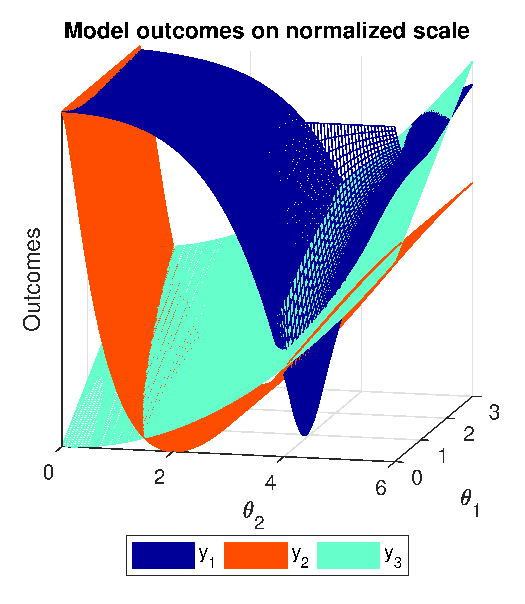
\includegraphics[width=.4\linewidth]{FIG_toy_sim_model_outputs.eps}
%\captionsetup{width=.4\linewidth}
\caption{Example model outputs shown on a common scale.}
\label{fig:toy_sim_outputs}
\end{figure}
%
%For CDO, the true function was used (rather than a GP emulator). 
%For CDO, a budget of 432 model observations was used. 
%%
%These were drawn as a full factorial design on a $3\times12\times12$ evenly-space grid over the supports of $x,\theta_1,\theta_2$. 
%%
%Using these model runs, the covariance function parameters $\lambda_\eta,\boldsymbol \beta^\eta$ in (\ref{eq:Hig_cov}) were set to their MLEs: $\lambda_\eta = 8.37\cdot10^{-4}$, $\boldsymbol\rho^\eta = [0.281, 0.999, 0.600, 0.720, 0.103]$ where $\rho^\eta_k = \exp(-\beta_k^\eta/4)$. 
%Thus we have 
Assuming an easily evaluated model, we have
%
$
\mathbf y(\mathbf x, \boldsymbol\theta) = \mathbf f(\mathbf x,\boldsymbol \theta) + \delta(\mathbf x) + \epsilon
$
%
for desired observation $\mathbf y$, where $\mathbf f$ is the model output, $\delta(\cdot)$ is the discrepancy function and $\epsilon$ is $N(0,0.05)$.

We initially set the desired observations to $[0,0,0]$, constant as a function of $x$. 
%
We then estimated the Pareto front via a preliminary round of CDO in order to estimate the standardized distance of the desired observation from the Pareto front.
%
The distance from the estimated Pareto front to the desired observation was found to be large -- at 16 units on the standardized scale, roughly four times the diameter of the entire model range.
%
As a result, the use of $[0,0,0]$ as a desired observation would lead to poor identifiability of the optimal region. 
%
This is because the desired observation is approximately the same distance from any point in the model range, relative to the distance from the desired observation to the optimal region.
%
%Therefore in order to improve identifiability of the optimal region, we updated the desired observation to lie closer to the estimated Pareto front (along the same line connecting to the orginal desired observation).
Therefore in order to improve identifiability of the optimal region, we updated the desired observation to lie along the same line connecting the original desired observation to the estimated Pareto front, but now closer to the latter.
%
We chose a distance of one unit away (roughly one fourth of the diameter of the model range), approaching the estimated Pareto front as closely as possible while remaining confident that the new desired observation of $[0.71, 0.71, 17.92]$ still outperforms the true Pareto front (i.e., lies outside the model range and is such that if it were added to the model range, it would be a Pareto optimal point).
%
We then set the discrepancy marginal precision $\lambda_\delta$ to 1 for subsequent CDO, corresponding to a degenerate prior informed by the estimated distance of the new desired observation from the Pareto front.
%
Observation error $\epsilon(\cdot)$ from \eqref{eq:model_gen} was taken to be distributed as $N(0,0.05)$ for all $x$.
%
Figure \ref{fig:toy_sim_results} shows the resulting posterior distribution, including the marginal distributions of the calibration parameters. 
%
The sharply peaked marginals show substantial Bayesian learning compared to the prior distributions distribution of the calibration parameters, which is uniform over the area shown in the scatterplot. 
%
The calibration successfully maps the contours of the optimal region, and peaks near the true optimum. 
%
%Among the posterior predictive samples $\tilde {\mathbf y}$ associated with each draw of $\boldsymbol \theta$, $91.9\%$ lie within two standard deviations of the true optimum.

\begin{figure}
\centering
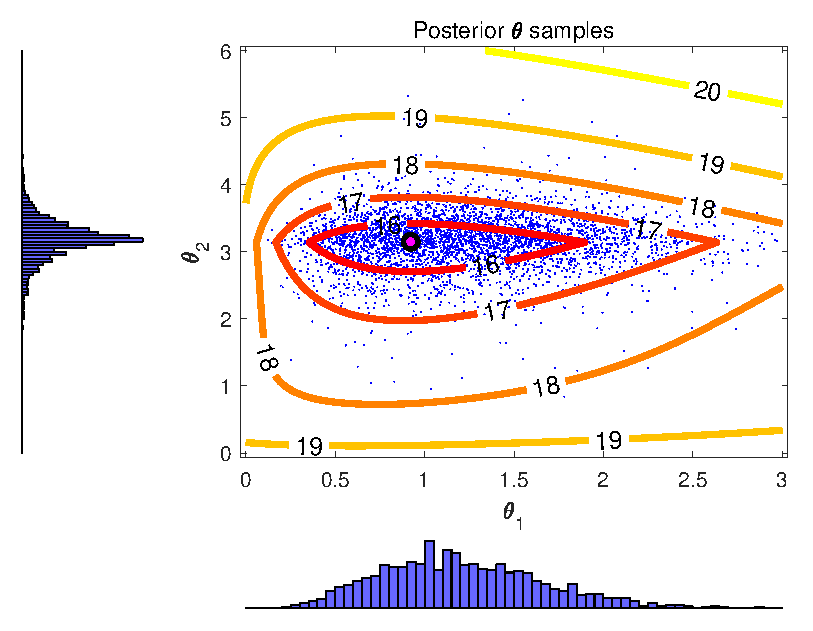
\includegraphics[scale=.8]{FIG_post_theta_contour_desobs0_lambdadelta1}
%\captionsetup{width=.7\linewidth}
\caption{Posterior draws from CDO in the simulated example. The contours show, for each point in the parameter space, the Euclidean distance of the model output at that point from the desired observation (averaged across the control input range $[1.95,2.05]$). The large dot shows the true optimum.}
\label{fig:toy_sim_results}
\end{figure}



\section{Application}\label{application}

In this section we describe the use of CDO for designing a material to be used in a wind turbine blade of fixed geometry. 
%
In traditional engineering design, material selection is a matter of choosing a material with appropriate properties for the project at hand from a database of known materials, often as a matter of ad-hoc satisficing. 
%
Material design usually occurs separately, and without an eye to specific end-uses. 
%
CDO allows us to wed these design processes, selecting a material design by modeling its performance outcomes in a wind turbine blade.
% particular engineering application. 
%
%Therefore, here we offer an example of calibrating material design parameters to desired performance targets for a wind turbine blade. 
%
This calibration is mediated by a model using \texttt{ANSYS} finite element analysis software. 
%
The finite element model is treated as an accurate representation of reality. %In this section I describe the emulator, and in Section \ref{MCMC} I describe its use for the calibration procedure.

\subsection{Project background}

Two primary performance targets for the design and construction of wind turbine blades are the distance (in meters) that the blade tip deflects under load from its starting position, and the angle of rotation the blade experiences under load.
%
Within the set of materials studied here, we want each of these measures and the material cost be as close to zero as possible.
%
The blade is to be a composite of two given materials, one serving as the \textit{matrix} and the other the \textit{filler}. 
%
In a composite, the matrix holds the filler together; an example would be concrete, in which a filler of loose stones is combined with a matrix of cement.
%
For the wind turbine blade, given a fixed choice of matrix and filler, the properties of the composite depend on the volume fraction (i.e. the volume ratio of filler material to matrix material used in the composite) and the thickness of the material used to build the blade. 
%
The resulting material properties impact the performance of the blade, as well as its cost per square meter. 
%
The finite element model takes as inputs a triplet $(h,v,k)$, where $h$ is the operating temperature of the wind turbine (in kelvin), $v$ is the volume fraction of the material, and $k$ is the thickness of the material (in mm). 
%
The outputs of the model are a triplet $(d,r,c)$, where $d$ is tip deflection (in meters), $r$ is rotation (in radians), and $c$ is cost per square meter (USD).
% 
The wind turbine should be capable of operating over the range of temperatures 230K-330K. 
%
We used CDO to find a distribution on optimal settings for $v$ and $k$ given outputs from the finite element simulator and desired observations.

\subsection{Emulation of finite element model}\label{emulator}
The finite element simulator is too computationally expensive to be suitable for direct use in (e.g.) an MCMC routine. 
%
We employed a GP emulator in the manner of \cite{Williams2006}. 
%
For this purpose, we drew 504 (trivariate) observations from the finite element simulator. 
%
These inputs follow a Latin hypercube sampling design \citep{McKay1979} based on plausible ranges for the three inputs, as identified by subject matter experts.
%
We consider the finite element observations to follow a GP with mean 0 and covariance function $C$ as described by (\ref{eq:Hig_cov}) above, with $\alpha_\eta=2$. 
%
This choice of $\alpha_\eta$ assumes smooth, infinitely differentiable sample paths. 
%
%I do not include a discrepancy function, per the considerations of Section \ref{obs_error}.

The hyperparameters $\lambda_\eta,\boldsymbol \beta^\eta$ must be estimated.
% 
To avoid our estimates being biased by calibration to the desired observations, we estimated them prior to calibration via maximum likelihood estimation.
% 
%Initially, a grid optimization method was used: a grid of $\boldsymbol \beta^\eta$ values was used, finding at each point of the grid the likelihood of the simulation observations integrated over the support of $\lambda_\eta$. 
%
%However, $\boldsymbol \beta^\eta$ is a five-dimensional vector, and a grid fine enough to be useful was too computationally burdensome to be feasible. Instead, a 
We used \texttt{fmincon()} in {\sc Matlab} %\citep{Cauchy1847} 
to maximize the log-likelihood of the simulation observations  (Equation \eqref{eq:full_dist} with $\mathcal D=\boldsymbol\eta$) over the joint (6-dimensional) support of $\boldsymbol \beta^\eta,\lambda_\eta$.  
%
The result is $\hat\lambda_\eta = 0.0152$, $\boldsymbol {\hat\rho}^\eta = (0.9358, 0.6509, 0.6736, 0.4797, 0.9673)$
%\begin{equation}\label{eq:MLEs}
%\boldsymbol {\hat\rho}^\eta = (0.9358, 0.6509, 0.6736, 0.4797, 0.9673),\quad
%\hat\lambda_\eta = 0.0152
%\end{equation}
where $\rho^\eta_k = \exp(-\beta_k^\eta/4)$. 
%A slice of the resulting emulator mean (for thickness = 20mm) for the tip deflection output is shown in Figure \ref{fig:emulator_surface}.

%\subsubsection{Wind turbine blade simulator}
%% Here the finite element model will be described
%Blah
%
%\subsubsection{Mathematical basis for the emulator}
%% Includes formulae for trained mean and covariance functions
%Blah
%
%\subsubsection{Experimental design}
%% How we selected the design points at which to observe the simulator
%Blah
%
%\subsubsection{Covariance parameters}
%% How they were selected
%Blah

%\paragraph{Finding covariance parameters via MCMC}
%% Why we didn't do it (computational difficulties
%Blah
%
%\paragraph{Grid optimization}
%% Advantages and disadvantages; full grid and integration of lambda
%Blah
%
%\paragraph{Gradient method}
%% Explanation and advantages
%Blah

%\begin{figure}
%\centering
%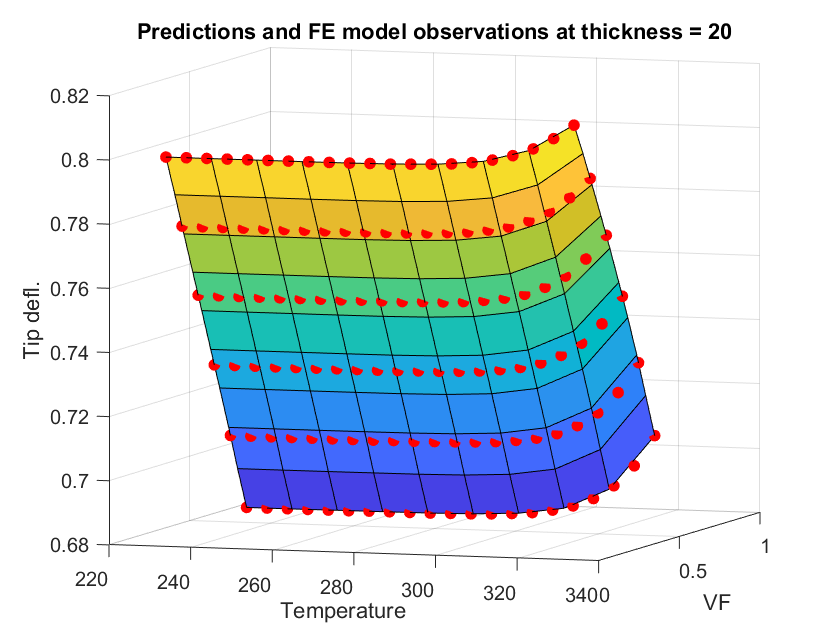
\includegraphics[width=.65\linewidth]{emulator_surface}
%\captionsetup{width=.65\linewidth}
%\caption{A slice of the GP emulator mean (restricted to the output for tip deflection) at thickness = 20mm. Red dots are observations from the simulator.}
%\label{fig:emulator_surface}
%\end{figure}

%\subsection{MCMC methods}
%% Background on MCMC
%Blah

\subsection{Calibration of the wind turbine blade system}\label{the_model}
% Choice of priors and resulting likelihood
%The model takes the trained emulator to be distributed as
%
%\begin{equation}\label{posterior_GP}
$
%\mathcal {GP}\left(\mu^*(\mathbf b), C^*(\mathbf b,\mathbf b')\right),
$
%\end{equation}
%
%where $\mu^*(\mathbf b) = \mathbf C_{\mathbf b,\mathbf B} \cdot \mathbf C_{\mathbf B,\mathbf B}^{-1} \cdot \boldsymbol \eta$, $C^*(\mathbf b,\mathbf b') = \mathbf C_{(\mathbf b^T,\mathbf b'^T)^T,(\mathbf b^T,\mathbf b'^T)^T} - \mathbf C_{(\mathbf b^T,\mathbf b'^T)^T,\mathbf B}\cdot \mathbf C_{\mathbf B,\mathbf B}^{-1} \cdot \mathbf C_{\mathbf B,(\mathbf b^T,\mathbf b'^T)^T}$, $\mathbf C_{\Upsilon,\Gamma}$ is the matrix whose $i,j$ element is equal to the covariance between the observation at the $i^{\text{th}}$ row of $\Upsilon$ and at the $j^{\text{th}}$ row of $\Gamma$, $\mathbf b=(\mathbf x,\mathbf t)$ is a row vector of control and calibration inputs, $\mathbf B=(\mathbf b_1^T,\mathbf b_2^T,\cdots,\mathbf b_n^T)^T$ is the $1512\times5$ matrix of locations of the 1512 simulation observations, and $\boldsymbol\eta$ is a column vector of the 1512 simulation responses: $\eta_i=\eta(\mathbf b_i)$. 
%
All model inputs were normalized to [0,1] over their supports. 
%
All model outputs were standardized so that the vector of simulation responses $\boldsymbol\eta$ has mean 0 and standard deviation 1.
%
%$C(\cdot,\cdot)$ is given by (\ref{eq:Hig_cov}), where we plug in the MLEs given above. 
%
The full joint posterior density of the calibration parameters and discrepancy function hyperparameters is given in Equation \eqref{eq:full_dist}, using the MLEs given above.%, is
%\begin{equation} \label{eq:wt_full_dist}
%$
%\pi(\boldsymbol\theta,\lambda_\delta,\boldsymbol\rho^\delta|\mathcal D) 
%\propto 
%\pi(\mathcal D|\boldsymbol\theta,\lambda_\delta,\boldsymbol\rho^\delta)
%\times
%\pi(\lambda_\delta)
%\times
%\pi(\boldsymbol\rho^\delta).
%$
%\end{equation}
%

The initial desired observations were set to $[0,0,0]$ on the original scale, constant as a function of temperature, on a grid of temperature values.
%
We carried out an initial round of CDO in order to update the desired observations to ones that lie close to the Pareto front.
%
For this purpose, a total of 20,000 samples were drawn via Metropolis-Hastings-within-Gibbs MCMC, of which 4,000 samples were discarded as burn-in. 
%
During the burn-in period, the covariance of the proposal distributions for $\boldsymbol \theta$, $\lambda_\delta$, and $\boldsymbol\rho^\delta$ were all periodically adjusted for optimal acceptance rates using the sample covariance of the preceding draws.
%
%The adjustment took place every 100 iterations of the MCMC, at which point the relevant covariance matrix was set to be equal to the sample covariance of the previous draws, times a scalar multiplier. 
%
%The level of the scalar multiplier was adaptively adjusted to promote optimal acceptance rates of $\approx 30\%$ for $\boldsymbol\theta$ and $\boldsymbol\rho$, and $\approx 44\%$ for $\lambda_\delta$.
%
As expected for the preliminary round of CDO, the posterior distribution of $\boldsymbol\theta$ was quite diffuse.
%
We used the GP emulator to estimate the model output for each sample of $\boldsymbol \theta$ drawn.
%
We filtered the resulting posterior predictions to retain only the estimated Pareto front.
%
Examining the estimated Pareto front, one finds a distinct ``elbow''; see figure \ref{fig:elbow}.
%
\begin{figure}
\centering
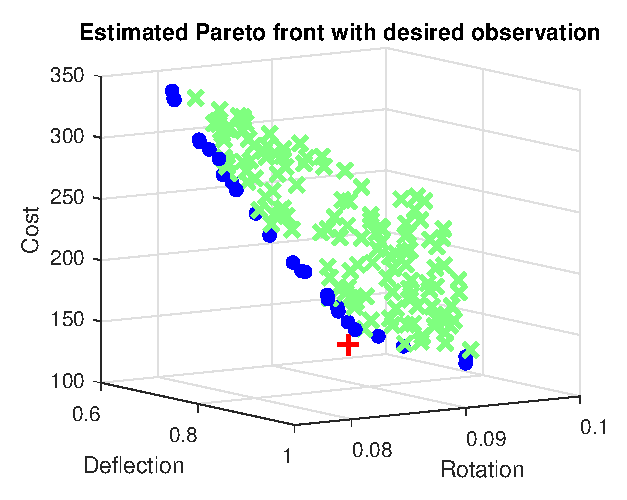
\includegraphics[scale=0.8]{FIG_est_PF_with_des_obs.eps}
%\captionsetup{width=.7\linewidth}
\caption{Each x shows a non-Pareto optimal point drawn from the predictive distribution through preliminary CDO. The dots show the estimated Pareto front. The plus sign is the desired observation selected to calibrate to the ``elbow'' in the Pareto front.}
\label{fig:elbow}
\end{figure}
%
We selected this elbow as the target for calibration.
%
To do so, we set the point $[\mathrm{deflection}=0.75\mathrm m,\ 
\mathrm{rotation}=0.09\ \mathrm{rad},\ 
\mathrm{cost}=\$130.34]$
 as the desired observation (constant as a function of temperature).
%
The elbow is the closest region of the Pareto front to this point.
%
Based on the estimated Pareto front, the desired observation is approximately 0.2 units away on the standardized scale.
%
Therefore, we set $\lambda_\delta=1/0.2^2=25.$
%

In the resulting CDO, we employed the same MCMC approach as in the preliminary round, except that $\lambda_\delta$ was now treated as known.
%
The marginal posterior distribution of the calibration parameters is shown in Figure \ref{fig:wt_marg_post} via four levels of highest density regions.
%
The contrast of the posterior distribution with the prior, which is uniform over the area shown in the figure, indicates that significant Bayesian learning has occurred in the calibration process.
%
%\begin{figure}
%\centering
%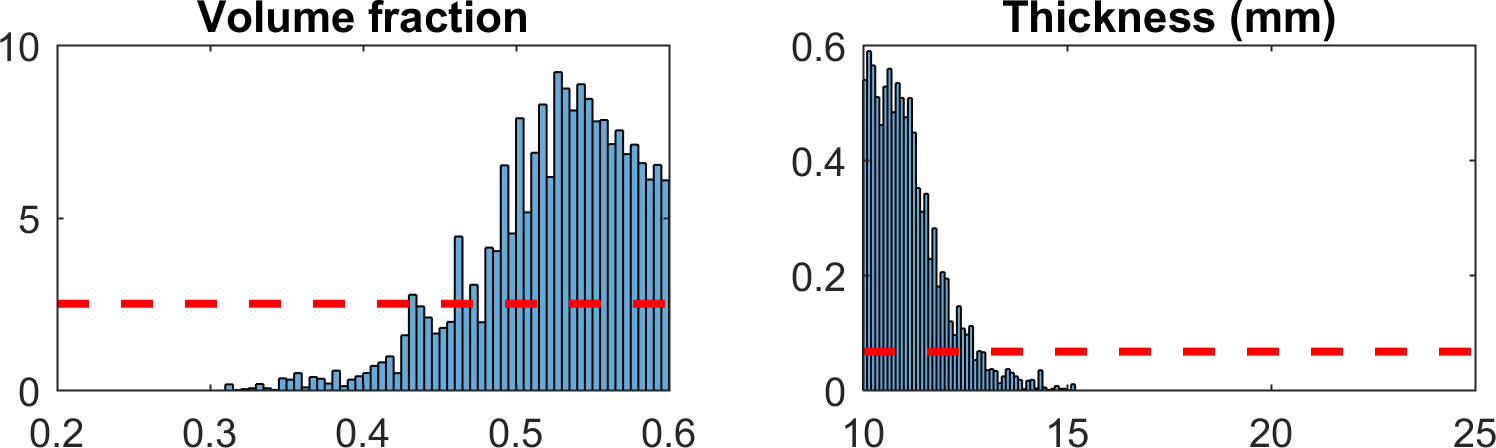
\includegraphics[width=.7\linewidth]{FIG_posterior_marginals_with_priors}
%\captionsetup{width=.7\linewidth}
%\caption{The histograms show the marginal posterior of each calibration parameter. The dotted lines show the priors.}
%\label{fig:wt_marg_post}
%\end{figure}
\begin{figure}
\centering
%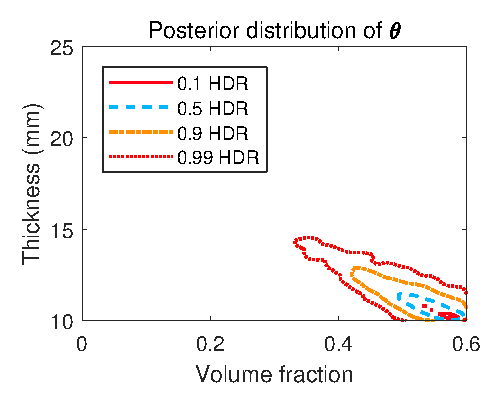
\includegraphics[width=.4\linewidth]{FIG_post_dist_contourplot}
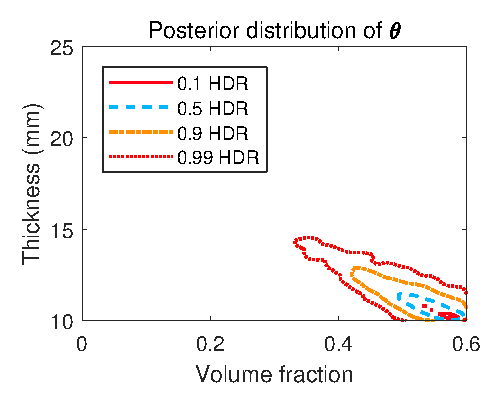
\includegraphics[scale=0.8]{FIG_post_dist_contourplot}
%\captionsetup{width=.7\linewidth}
\caption{Four levels of highest density regions of the posterior distribution from calibration of the wind turbine blade system. The prior is uniform over the area shown.}
\label{fig:wt_marg_post}
\end{figure}
%
The prior and posterior marginal predictive distributions of the model outputs are shown in Figure \ref{fig:prior_post_pred_comp}.
%
\begin{figure}
\centering
%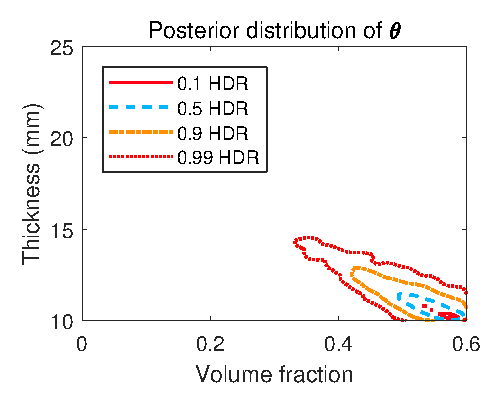
\includegraphics[width=.4\linewidth]{FIG_post_dist_contourplot}
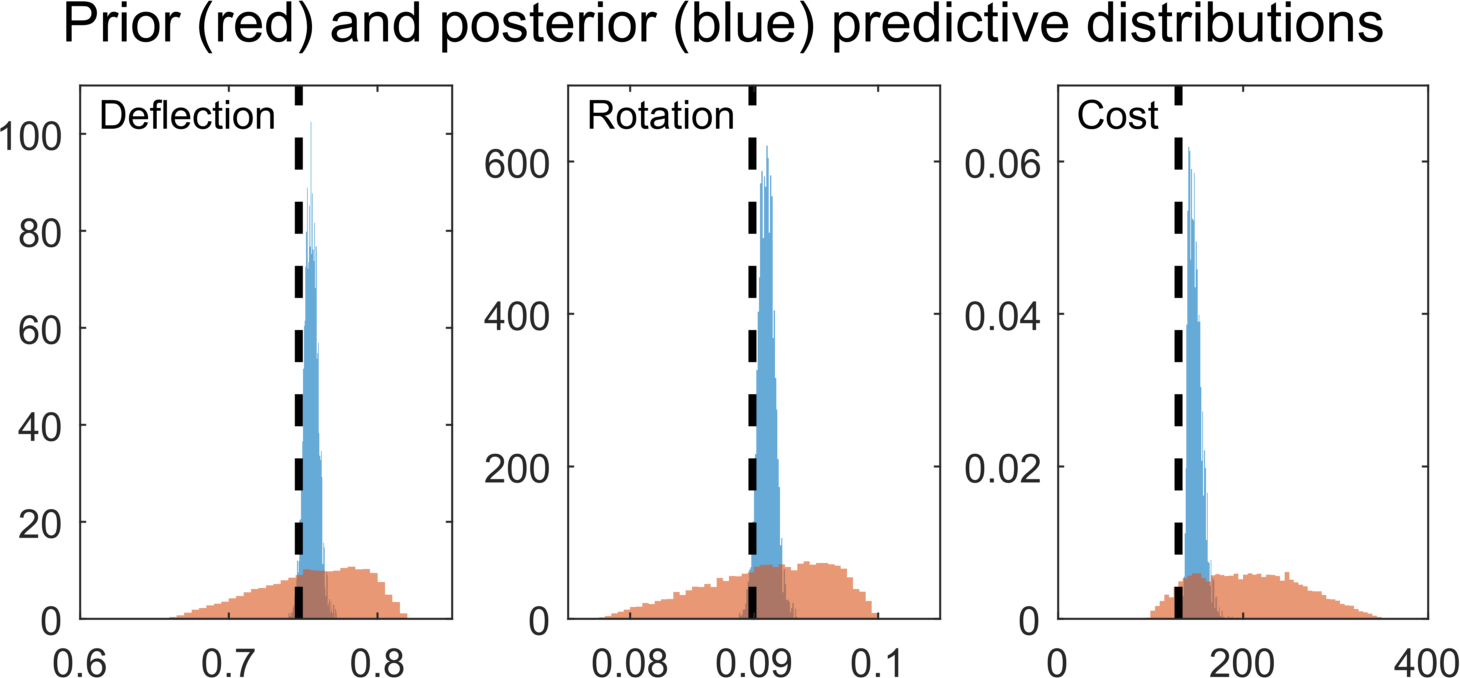
\includegraphics[scale=0.8]{FIG_prior_vs_posterior_dist}
%\captionsetup{width=.7\linewidth}
\caption{Prior and posterior marginal predictive distributions for each of the three model outputs. Notice that it is to be expected that the posteriors peak near the target (and not on it), since the target was intentionally chosen to lie outside the model range.}
\label{fig:prior_post_pred_comp}
\end{figure}
%
The posterior marginals peak sharply near the performance target.
%
The mean model output under the prior is $[\text{deflection}=0.76\mathrm m,\ \text{rotation}=0.09\text{ rads},\ \text{cost}=\$207.90/\mathrm m^2]$, whereas under the posterior it is $[0.76\mathrm m,0.09\ \mathrm{rad},\$148.68]$.
%
Though the performance outcomes are approximately the same under the posterior distribution as under the prior, the cost per square meter has dropped dramatically.
%
If one desires instead to prioritize gains in performance over cost, this can be accomplished by selecting desired observations that reflect those priorities. 

\subsection{Pareto front estimation}\label{removing_cal_pars}

%\subsubsection{Motivation}

Often in the case of a system with multivariate output, one might not antecedently have a clear target outcome.
%
When \textit{ceteris paribus} all outputs are to be minimized, any point in the Pareto front is optimal relative to some set of priorities.
%
If those priorities have not been explicitly determined prior to calibration, then no particular outcome can be targeted.
%
In determining one's priorities, it is helpful to know the Pareto front of the relevant system.
%
For example, in a system where quality is monotonically increasing in cost, depending on one's tolerance for high cost, any point in the model range might be optimal.
%
%In determining one's priorities and selecting a target outcome, it is valuable to have a clear and accurate understanding of the Pareto front of the system.
%
In low-dimensional cases, CDO may be used to achieve a holistic picture of the Pareto front by optimizing to each of a grid of performance targets.
%
%Where a model contains several outputs that one wishes to optimize, it can become complicated to juggle one's priorities in selecting targets for each of these outputs.
%
%Again to speak from the wind turbine application: we know we want to keep cost, deflection, and rotation low, but we might not have a clear prior conception of exactly what sorts of trade-offs amongst those outcomes we would consider optimal, much less how to implement our priorities in the calibration procedure. 
%
%Rather than wishing to optimize relative to some particular set of desired observations, one may prefer simply to learn as much as possible about the Pareto front as a whole.
%
%In low-dimensional cases this may be achieved using CDO as follows.
%
To do this, where the model output is $d-$dimensional, one may draw a grid over the range of $d-1$ of the model outputs and perform CDO to minimize the remaining output at each point of the grid.
%
The $d-1$ outputs, at each grid point, are treated as known up to observation error (meaning that the discrepancy function $\delta(\cdot)$ is set to 0 in the dimension of these outputs).
%
The resulting estimate is distinguished from other methods of estimating the Pareto front (including from the filtering method employed in preliminary CDO) by including uncertainty quantification.
%

This procedure is illustrated here using the wind turbine blade application.
%
For simplicity, rotation has been removed as a model output, leaving a system with 2-dimensional output of deflection and cost. 
%
The range of cost is known (via preliminary CDO) to be $[\$96,\$352]$.
%
A 20-point grid was drawn over this range of costs. 
%
%Using the rough estimate of the Pareto front from preliminary CDO, we found that to cover the Pareto front, the cost grid should cover the range $[\$96,\$352]$.
%
For each point $c$ in the cost grid, we used the point $(0\mathrm m,\$c)$ as the performance target for calibration (constant with respect to temperature).
%
For each such point, we then updated this initial desired observation to improve identifiability using the rough estimate of the Pareto front from preliminary CDO using desired observation $(0\mathrm m,\$0)$.
%
Note that only one round of preliminary CDO was needed for this purpose, rather than a separate instance at each grid point.
%
%, to be a point which lies near the Pareto front, to improve identifiability.
%
%Here as in Section \ref{the_model}, ``near'' was taken to be 0.2 units on the standardized scale of model outputs.
%

%\paragraph{Specifying known cost}\label{known_cost}
%
%The above strategy of performing the calibration across a grid and forming a response surface over that grid may be applied even more directly, to largely the same end as in the previous section. Namely: rather than replace one or more desired outputs with a prior on the calibration inputs and drawing a grid over the hyperparameter(s) of that prior, one can instead simply draw a grid over one or more of the desired outputs, treating those outputs as known up to slight deviations at each point of the grid. This strategy has the advantage that, unlike the above strategy, it does not require that we have prior knowledge of any relationship between the calibration parameters and the outputs. Furthermore, whereas the previous strategy requires removing a model output, the current strategy uses the same version of the model, relying solely on changes to the desired observations and observation variance to effect the strategy. In comparison with the previous section's strategy, the approach in the current section also enjoys better interpretability.
%
%For convenience, call an output that is specified as known up to slight deviations in the way suggested here ``d-known''. To specify an output as d-known, it suffices to (1) choose a desired observation of that output which is realistically achievable, and (2) set a constant, low observation variance for that output. The precise value of the observation variance for a d-known output can be tuned during the burn-in period of the MCMC routine. It ought to be as low as possible while still allowing for healthy mixing in the MCMC. If the variance is too small, then proposed draws of the calibration parameters will be likely to take the model output too far away from the d-known output, resulting in the draw being rejected, and hence low acceptance rates and poor mixing.
%
%The other desired observations -- those that are not d-known -- can be treated as usual, with their observation variances each drawn from a $1/\sigma^2_i$ prior, or whichever other treatment of observation variance from Section \ref{des_obs_var} one wishes to use. Thus at the calibration procedure which takes place at each point in the grid of d-known outputs, the d-known outputs have in essence been removed from the CDO, and are treated as known up to a slight variance for facilitating healthy MCMC. This ``removal'' requires little modification to the model, but still serves to simplify the choice of desired observations and observation variance. 
%
%The full model is given by
%\begin{equation}\label{full_model_3}
%\begin{aligned}
%\pi(\boldsymbol\theta,\mathbf C_{\mathbf y}|\mathcal D ) &\propto
%\pi(\mathcal D|\boldsymbol\theta,\mathbf C_{\mathbf y}) \times \pi(\boldsymbol\theta) \times \pi(\mathbf C_{\mathbf y})\\
%&\propto  \pi(\mathcal D|\boldsymbol\theta,\mathbf C_{\mathbf y}) \times \pi(\mathbf C_{\mathbf y})\\
%&\propto \lvert \mathbf C_{\mathcal D} \rvert ^{-1/2} \mathrm{exp}(\mathcal D^T \mathbf C_{\mathcal D}^{-1} \mathcal D) \times \prod_{i=1}^2 \frac1{\sigma^2_i}
%\end{aligned}
%\end{equation}
%where $\mathbf C_{\mathbf y}$ is the diagonal matrix where the $j,j$ entry $c_j$ is equal to $\sigma^2_1$ if $y_j$ is an observation of deflection, $c_j=\sigma^2_2$ if $y_j$ is an observation of rotation, and $c_j = s$ if $y_j$ is an observation of cost, for some small pre-selected value of $s$. In this application, I set $s=0.05$, so that the observation variance on standardized cost values at each point of the grid was 0.05. 

%The result of this strategy is similar to that one can derive a response surface over the $d-1$-dimensional grid of outputs, where that response describes the optimal results across the grid. 
%
%If the grid covers the Pareto front in $d-1$ dimensions, then t
The result of the strategy is to provide an estimate of the response surface with included uncertainty quantification describing, for each point in the grid, the optimal achievable outcome for the output not included in the grid.
%
Thus a decisionmaker can visualize the space of desirable possibilities with associated uncertainty metrics. 
%
They can do so without the need for antecedently rigorously determining their exact priorities for weighing gains in each of the outputs against one another.
%, nor (much worse) working out how to translate those priorities into specific choices of desired observations and observation variance schemes. 
%This is similar to the strategy of the previous section, but in addition to other benefits, this result has better interpretability in that the grid is over one of the model outputs, rather than over a hyperparameter whose interpretation is somewhat dubious. For example, a decision-maker is likely to feel quite comfortable choosing a budget based on expected outcomes at each cost; they may be less comfortable selecting a value of $\lambda_{cost}$.

%The same sort of uncertainty analysis described in Section \ref{non-uniform_prior} is available here, since posterior parameter uncertainty and code uncertainty are easily recovered from the results of the MCMC routine. 
%
The result of applying this strategy to the wind turbine blade application is shown in Figure \ref{fig:known_cost}. 
%
The lefthand plot shows that the posterior model output respected the ``known'' cost values used in the calibrations.
%
The Pareto front for the system appears with uncertainty bands in the righthand plot.
%
This plot visualizes a distribution on the optimal performance outcome for any cost that a decisionmaker might select as a budget for production, which would be helpful when selecting a budget.
%
For example, the elbow around \$140 manifests itself as a potentially attractive choice, since it can be seen in the plot that prior to that point each dollar spent brings significant gains in reducing deflection.
%
Spending above that level continues to reduce deflection, but less sharply.


\begin{figure}
\centering
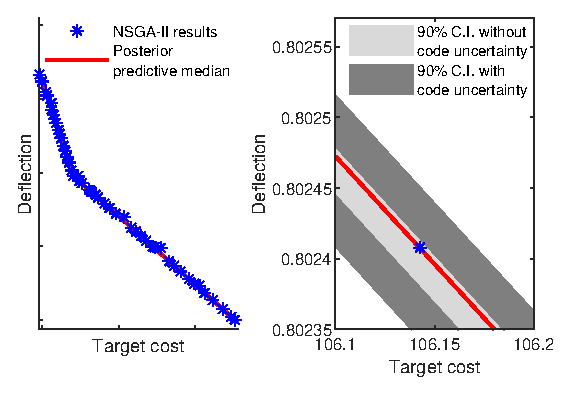
\includegraphics[scale=.8]{FIG_cost_grid_pareto_bands.eps}
%\captionsetup{width=.7\linewidth}
\caption{The lefthand plot verifies that the calibration achieved the ``known" costs up to small error. The righthand plot is an estimate of the Pareto front for the system with attendant uncertainty quantification.}
%\caption{The righthand plot shows ``Pareto bands'' of wind turbine blade posterior cost and tip deflection across a range of target costs. The gray region gives a 90\% credible interval only considering parameter uncertainty; the blue region extends this to include code uncertainty.}
\label{fig:known_cost}
\end{figure}




\section{Conclusion} \label{conclusion}
% Discussion of the role of computer model validation as a potential methodology for design

We have described the 
%theoretical background for the use of Gaussian processes to emulate computationally expensive computer model code, and the 
use of computer model calibration under the framework established by \cite{Kennedy2001}, \cite{Williams2006} and \cite{Bayarri2007} and how it can be used to address questions of engineering design. 
%
CDO is a modification of that framework which calibrates a computer model, not to field observations, but rather to desired observations; i.e., to performance targets for the system. 
%
Unlike other methods of Bayesian optimization (e.g., \citealt{Shahriari2016}), CDO does not require the ability to carry out computer model observations adaptively.
%
Instead, it can operate using a batch of observations gathered prior to (and independently of) the calibration procedure.
%
We described the implementation of this approach in an MCMC routine along with considerations to accommodate computational instability.
%
The use of this methodology is illustrated in the case of material design for a wind turbine blade. 

We have shown thereby a variety of ways in which CDO can be used to guide decision-makers in the design process. 
%
By expropriating established tools of model calibration, CDO offers a method of optimization which is sensitive to all sources of uncertainty, and which results in an estimate that includes uncertainty quantification.

As discussed earlier, the methodology as described here treats the computer model as universally valid over the domain of the calibration inputs. 
%
Future work in this area will include the use of a discrepancy term capturing model bias.
%
This would allow for simultaneous calibrations: both traditional and CDO.
%
That is, a computer model could be calibrated to real observations while also being calibrated to performance targets treated as desired observations.
%
These two goals would not necessarily conflict, since the two calibrations take different inputs to be the calibration parameters.
% 
CDO calibrates inputs that are under operator control, and thereby would be treated as control inputs in traditional calibration.
%
Other extensions of the proposed methodology could include its application to state-aware calibration \citep{Atamturktur2015,Stevens2018,Brown2016}, which would allow the optimal region of the calibration parameters to vary as a function of the control inputs.



\bigskip
\begin{center}
{\large\bf SUPPLEMENTARY MATERIAL}
\end{center}

\begin{description}

%\item[Title:] Brief description. (file type)

\item[\scshape{Matlab} code for CDO:] This includes the example model described in Section \ref{example}, along with code to perform CDO on that system and thereby reproduce Figure \ref{fig:toy_sim_results}.

%\item [{\fontfamily{cmu}\selectfont \sc Testing} code for CDO:] This includes

%\item[R-package for  MYNEW routine:] R-package �MYNEW� containing code to perform the diagnostic methods described in the article. The package also contains all datasets used as examples in the article. (GNU zipped tar file)
%
%\item[HIV data set:] Data set used in the illustration of MYNEW method in Section~ 3.2. (.txt file)

\end{description}

\bibliographystyle{Chicago}

\bibliography{lit_review}
\end{document}

\begin{figure}
\begin{center}
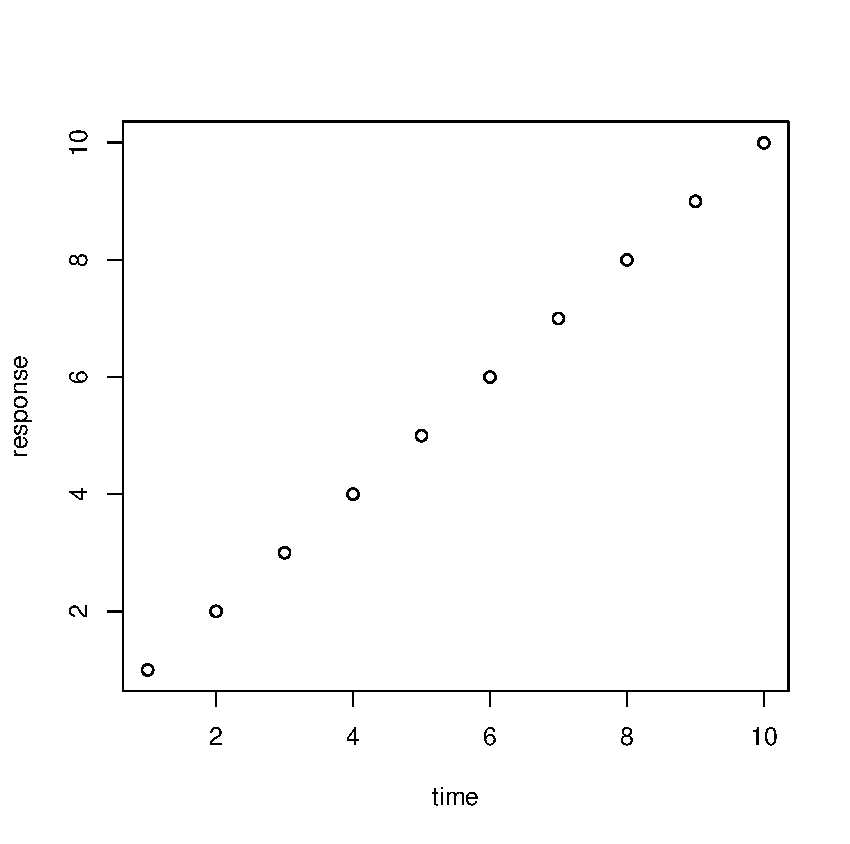
\includegraphics[width=3in]{fig1.pdf}
\end{center}
\caption{Consistency comparison in fitting surrogate model in the tidal
power example. \label{fig:first}}
\end{figure}

\begin{table}
\caption{D-optimality values for design $X$ under five different scenarios.  \label{tab:tabone}}
\begin{center}
\begin{tabular}{rrrrr}
one & two & three & four & five\\\hline
1.23 & 3.45 & 5.00 & 1.21 & 3.41 \\
1.23 & 3.45 & 5.00 & 1.21 & 3.42 \\
1.23 & 3.45 & 5.00 & 1.21 & 3.43 \\
\end{tabular}
\end{center}
\end{table}

\begin{itemize}
\item Note that figures and tables (such as Figure~\ref{fig:first} and
Table~\ref{tab:tabone}) should appear in the paper, not at the end or
in separate files.
\item In the latex source, near the top of the file the command
\verb+\newcommand{\blind}{1}+ can be used to hide the authors and
acknowledgements, producing the required blinded version.
\item Remember that in the blind version, you should not identify authors
indirectly in the text.  That is, don't say ``In Smith et. al.  (2009) we
showed that ...''.  Instead, say ``Smith et. al. (2009) showed that ...''.
\item These points are only intended to remind you of some requirements.
Please refer to the instructions for authors
at \url{http://www.tandfonline.com/action/authorSubmission?journalCode=utch20&page=instructions#.UieFdDafgx0}
\item If you have Supplementary Material (eg software, data, technical
proofs), identify them in the section below.  In early stages of the
submission process, you may be unsure what to include as supplementary
material.  Don't worry---this is something that can be worked out at later stages.
\end{itemize}
